\section{Attitude Determination and Control System (AOCS)}

\textbf{The payload onboard your satellite has a pointing requirement of 0,5°. You have to design a AOCS for the cubesat, with a budget of about 100 kEuros. The sensors and actuators that you can use are to be found on \url{https://www.cubesatshop.com/}}

\begin{itemize}
    \item[-] \textbf{Make a schematics diagram (such as the one found on slide 61 of “9-10.pdf”) of the AOCS control system with the (real) elements found here. } 

    \begin{figure}[h]
        \centering
        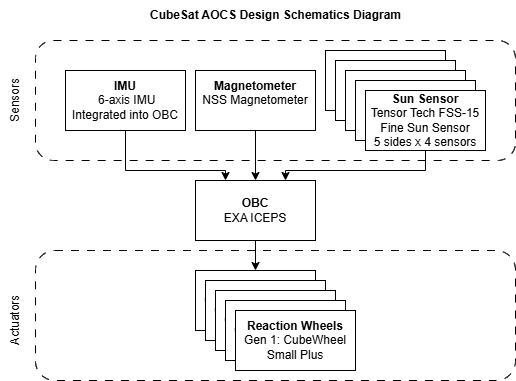
\includegraphics[width=0.8\linewidth]{Doc/Graphics/AOCS hardware diagram.png}
        \caption{CubeSat AOCS Design Schematics Diagrame made with draw.io}
        \label{fig:enter-label}
    \end{figure}

    \vfill
    
    \begin{table}[h]
        \centering
        \begin{tabular}{|l|c|c|c|c|}
        \hline
        \textbf{Position}&\textbf{Part Name}&  \textbf{Unit Price}&  \textbf{Amount}&  \textbf{Total Price}\\
        \hline \hline
        OBC / IMU&EXA ICEPS&  20 500€&  1&  20 500€\\ 
        Magnetometer&NSS Magnetometer&  15 000€&  1&  15 000€\\ 
        Sun Sensor&Tensor tech fine Sun Sensor& 1 800€& 4x4& 28 800€\\
        Reaction Wheels&CubeWheel small +& 6550€& 4& 26 200€\\
        Magnetorquers& EXA MT01 Compact Magnetorquer& 1200€& 4& 4 800€\\

        \hline
        & & & &\textbf{95 300€}\\ \hline
        \end{tabular}
        \caption{Cost estimation for CubeSat AOCS design}
        \label{tab:my_label}
    \end{table}


    \newpage
    \item[-] \textbf{Explain why you chose each element and how many of each are needed. }

    Since we are conducting a CubeSat mission which is being released from the ISS we can make a few assumptions about the requirements that will drive the design of the AOCS system.

    \textbf{Assumptions}
    \begin{itemize}
        \item \textit{CubeSat size:} Since the ISS CubeSat deployers (J-SSOD and NRCSD) seem to accomodate up to 6U \cite{deployers_wiki} cubesats and most recent CubeSats deployed from the ISS \cite{nanosats_database} have been up to 3U we will assume 3U as a reasonable size and design driver for the mission.
        This size limitation of 30cm x 30cm x 30cm for the CubeSat wall designs will dictate the size and amount of systems the satellite can accomodate

        \item Assuming the CubeSat is used for Earth-related observations or measurements, we will leave the Nadir face empty of AOCS systems to leave space for the payload.
        Thus, an earth sensor is out of question for attitude sensing.

        \item We also assume that we do not need to leave any budget margins or save any money to accommodate for possible cost overruns for the other satellite systems and as such can freely use the full 100 k€ budget.
    \end{itemize}

    \vspace{1cm}
    Based on these assumptions, we design the AOCS according to the needs of such a system and an ample amount of redundancy.
    
    \textbf{Needs:}
    \begin{itemize}
        \item \textbf{Attitude Sensors:}
        The AOCS needs both an internal and an external attitude sensor: one internal sensor for the CubeSat actuators to base their control algorithm on and an external sensor as a reference system. 
        I chose the \textit{EXA ICEPS Onboard Computer} as it contains a 6-axis Internal Measurement Unit.
        
        For the external sensor, I chose the \textit{NSS Magnetometer}. 
        This provides quite accurate external attitude measurements based on the Earth's magnetic field and it would be mounted on the outside of the CubeSat, however not on a Boom as it is optimised for, since it will work in complement with other sensors.
        
        To complement this sensor, I also added 4 \textit{Tensor Tech fine Sun Sensor} on the sun side of the CubeSat and three other sides (not the nadir side) to be mounted on the outside.

        \item \textbf{Attitude Actuators:}
        Since we might be dealing with an up to 6U CubeSat, I wanted to include a robust and fine actuation system to also comply with the pointing requirement of $0.5^{\circ}$. 
        For this purpose, I deemed reaction wheels the best choice. 
        I chose the 2nd smallest of the CubeWheel family, the \textit{CubeWheel Small +}. 
        The minimum requirement would be three of these and I chose 4 for redundancy.
        When using reaction wheels, it is also good practice to add external actuators to offload the wheels and thus enable a longer mission lifetime.

        I also added 4 \textit{EXA MT01 Compact Magnetorquers} as an external actuation method to complement the reaction wheels.

        \item \textbf{Redundancy:}
        Redundancy is present both in the amount of components chosen and the numbers of sensing methods and actuation.
        The OBC/IMU has 6 axis internal attitude sensing, providing at least one form of redundancy per axis. 
        The magnetometer provides no redundancy but serves as the main external attitude sensor and is proficiently radiation protected.
        
        The sun sensors provide an additional external attitude sensing method with plenty of redundancy with 1 extra sun sensor per side (minimum of three) and one redundant side mounted with the sensors.

        The reaction wheels include one additional wheel for redundancy (minimum of three) and external actuation methods with the magnetorquers to offload the reaction wheels. 
        The magnetorquers also include one redundant component (minimum of three)

        \item \textbf{Accuracy:}
        Given the chosen components and their accuracies, redundancies and error rates the pointing requirement of $0.5^{\circ}$ will be obtained.
    \end{itemize}
    
\end{itemize}

